\documentclass[conference]{IEEEtran}

\newcommand{\thetitle}{Non-Parametric Discrete Mixture Model Recovery via Nonnegative Matrix Factorization}

%!TEX root = paper.tex

\usepackage[labelfont=bf,small]{caption}
\usepackage[font=small,labelfont=bf,position=top,nearskip=0em]{subfig}
\usepackage{cite,amsmath,amssymb,rotating,multirow,bigstrut,url,wrapfig,relsize,paralist,array,mathtools,units}
\usepackage[hyperfigures,bookmarks,bookmarksopen,bookmarksnumbered,colorlinks,linkcolor=black,citecolor=black,filecolor=blue,menucolor=black,pagecolor=blue,frenchlinks=true,pdftitle={\thetitle}]{hyperref}

%!TEX root = paper.tex

%% LABELING COMMANDS
\renewcommand{\sec}[1]{\label{sec:#1}}
\newcommand{\eqn}[1]{\label{eqn:#1}}
\newcommand{\fig}[1]{\label{fig:#1}}
\newcommand{\tab}[1]{\label{tab:#1}}
\newcommand{\thm}[1]{\label{thm:#1}}
\newcommand{\defn}[1]{\label{def:#1}}

%% REFERENCING COMMANDS
\newcommand{\Appendix}[1]{\hyperref[sec:#1]{Appendix~\ref*{sec:#1}}}
\newcommand{\Section}[1]{\hyperref[sec:#1]{Section~\ref*{sec:#1}}}
\newcommand{\Equation}[1]{\hyperref[eqn:#1]{Equation~\ref*{eqn:#1}}}
\newcommand{\Figure}[1]{\hyperref[fig:#1]{Figure~\ref*{fig:#1}}}
\newcommand{\Table}[1]{\hyperref[tab:#1]{Table~\ref*{tab:#1}}}
\newcommand{\Theorem}[1]{\hyperref[thm:#1]{Theorem~\ref*{thm:#1}}}
\newcommand{\Definition}[1]{\hyperref[def:#1]{Definition~\ref*{def:#1}}}

%% MATHEMATICAL NOTATIONS

% common algebraic domains
\newcommand{\N}{\mathbb{N}}
\newcommand{\Z}{\mathbb{Z}}
\newcommand{\Q}{\mathbb{Q}}
\newcommand{\R}{\mathbb{R}}

% standard operators & functors
\renewcommand{\Pr}{\mathrm{Pr}}
\newcommand{\Image}{\text{Im}}
\newcommand{\Kernel}{\text{Ker}}

% common constructs
\newcommand{\abs}[1]{{\left|#1\right|}}
\newcommand{\absx}[1]{{|#1|}}
\newcommand{\card}[1]{{\left|#1\right|}}
\newcommand{\cardx}[1]{{|#1|}}
\newcommand{\norm}[1]{{\lVert#1\rVert}}
\newcommand{\normx}[1]{{\Vert#1\Vert}}
\newcommand{\set}[1]{{\left\{#1\right\}}}
\newcommand{\setx}[1]{{\{#1\}}}
\newcommand{\parens}[1]{{\left(#1\right)}}
\newcommand{\parensx}[1]{{(#1)}}
\newcommand{\bracket}[1]{{\left[#1\right]}}
\newcommand{\bracketx}[1]{{[#1]}}
\newcommand{\seq}[1]{{\left<#1\right>}}
\newcommand{\seqx}[1]{{\lvert#1\rvert}}
\newcommand{\tuple}[1]{{\left<#1\right>}}
\newcommand{\tuplex}[1]{{\lvert#1\rvert}}
\newcommand{\floor}[1]{{\left\lfloor#1\right\rfloor}}
\newcommand{\floorx}[1]{{\lfloor#1\rfloor}}
\newcommand{\ceil}[1]{{\left\lceil#1\right\rceil}}
\newcommand{\ceilx}[1]{{\lceil#1\rceil}}
\newcommand{\round}[1]{{\left[#1\right]}}
\newcommand{\roundx}[1]{{[#1]}}
\newcommand{\fracx}[2]{{#1/#2}}
\newcommand{\fracp}[2]{{\left(\frac{#1}{#2}\right)}}
\newcommand{\fracpx}[2]{{(#1/#2)}}
\newcommand{\smallfrac}[2]{{\textstyle{\frac{#1}{#2}}}}

% standard notations
\newcommand{\trans}[1]{{#1}^T}
\newcommand{\inner}[2]{{#1}\trans{#2}}
\newcommand{\cross}{\times}
\newcommand{\tensor}{\otimes}
\newcommand{\directsum}{\oplus}
\newcommand{\iso}{\cong}
\newcommand{\union}{\cup}
\newcommand{\inter}{\cap}
\newcommand{\Union}{\bigcup}
\newcommand{\Inter}{\bigcap}
\newcommand{\conj}{\wedge}
\newcommand{\disj}{\vee}
\newcommand{\Conj}{\bigwedge}
\newcommand{\Disj}{\bigvee}
\newcommand{\defeq}{=}
\renewcommand{\emptyset}{\varnothing}
\renewcommand{\setminus}{\,\raisebox{1pt}{$\smallsetminus$}\,}
\newcommand{\eldiv}{\,./\,}
\newcommand{\diag}{\text{diag}}
\newcommand{\rStoch}{\text{rs}}

%% FORMATTING BEHAVIORS
\newcommand{\caps}[1]{{\smaller{#1}}}
\newcommand{\latin}[1]{\textit{#1}}
\newcommand{\defterm}[1]{\textit{#1}}
\newcommand{\newfootnote}[2]{\newcommand{#1}{\footnote{#2} }}
\renewcommand{\bullet}{\raisebox{2pt}{$\centerdot$}}
\renewcommand{\arraystretch}{1.3}


\title{\vspace{-0.25em}\thetitle}
\author{
{\large{Stefan~Karpinski, John~R.~Gilbert, Elizabeth~M.~Belding}} \vspace{0.25em}\\
Department of Computer Science \\
University of California, Santa Barbara \vspace{0.35em}\\
\textit{\{sgk,gilbert,ebelding\}@cs.ucsb.edu}
}

\bibliographystyle{IEEEtran}

\newcommand{\figurename}{Figure}
\newcommand{\tablename}{Table}

\begin{document}
\maketitle

Mixture modeling expresses probability densities as convex combinations of constituent probability distributions:
\begin{align}\eqn{mixture-model}
  q_i(x) = \sum_{j=1}^r w_{ij} p_j(x),
\end{align}
Here $q_i$ and $p_j$ are density functions, and $w_{ij}$ are nonnegative weights, summing to unity for each $i$.
In classical mixture modeling, the constituent density functions, $p_j$, are assumed to be from some class of parametric distributions.
Various well established algorithms, using expectation minimization (\caps{EM}), can optimally recover the weights, $w_{ij}$, given an observed sample of values from $q_i$.

In certain settings, however, mixture modeling is desirable, but the constituent distributions are neither known in advance, nor can they be assumed to be parametric.
In this work, we demonstrate how, for discrete event spaces, nonnegative matrix factorization (\caps{NMF}) can be effectively used to simultaneously recover both weights and constituent distributions, given a large collection of variably-sized samples from mixtures.
% Our work addresses mixture models over discrete event spaces, but can be applied readily to continuous spaces, since continuous quantities can be discretized, and our techniques then applied to the resulting large discrete spaces. Since our approach makes no parametric assumptions, the results are no less valid.

For discrete event spaces, \Equation{mixture-model} is expressed succinctly as matrix multiplication.
Letting $Q_{ik} = q_i(k)$, $W_{ij} = w_{ij}$, and $P_{jk} = p_j(k)$ we have:
\begin{align}\eqn{mixture-model-matrix}
  Q = WP.
\end{align}
% The matrices are all be row-stochastic.
The problem of inferring both the weights, $w_{ij}$, and constituent distributions, $p_j$, from a collection of mixtures, $q_i$, is equivalent to finding the factors $W$ and $P$ given $Q$.
All three matrices are constrined to be row-stochastic, meaning that all entries are nonnegative, with rows summing to unity.

The problem of finding such a factorization is known as nonnegative matrix factorization.
Such factorizations are not unique, so perfect recovery of $W$ and $P$ cannot generally be achieved.
On the other hand, any exact factorization of $Q$, is an equally valid mixture model for the given data.
Since a variety of \caps{NMF} algorithms have been proposed, this problem is partially solved.
Several difficulties remain, however:
\begin{enumerate}
  \item $Q$ is not known exactly, only a finite sample for each distribution row of $Q$ is observed;
  \item The samples for the rows may not have uniform size;
  \item \caps{NMF} is known to be \caps{NP}-hard; thus, all efficient algorithms are heuristic, and may not yield adequate results.
\end{enumerate}
This list is not exhaustive, and we will address and discuss several further difficulties.

Our motivating application is mixture modeling for traces of network flows, whose distributions of packet sizes and inter-packet intervals can be effectively modeled as discretized mixture models, using \caps{NMF}~\cite{Karpinski08}.
In this setting, there are several particularly challenging aspects:
\begin{enumerate}
  \item The distribution of sample sizes is heavy-tailed, having a few very large samples, and many very small samples, with most flows having only one to three packets.
  \item The constituent distributions are not uniformly represented: the most prevalent distribution has much larger weights on average than the next, and so on.
\end{enumerate}
We will demonstrate using simulated data why both of these properties make factor recovery particularly difficult.

\begin{figure}[b]
\fig{synthetic-basis}
\begin{center}
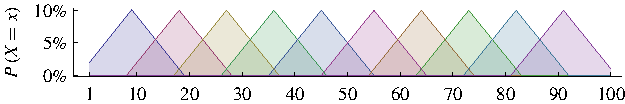
\includegraphics[width=3.5in]{synth/test}
\end{center}
\vspace{-0.7em}
\caption{Discrete distributions used to generate synthetic mixtures.}
\vspace{-0.5em}
\end{figure}

\begin{figure}[b]
\fig{synthetic-weights}
\begin{center}
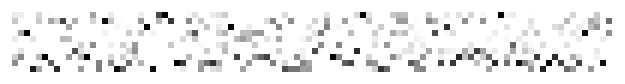
\includegraphics[width=3.5in]{synth/weights}
\end{center}
\vspace{-0.7em}
\caption{Transposed matrix plot of 100 sample random weights.}
\vspace{-0.5em}
\end{figure}

For synthetic data, we use saw-tooth patterns as constituent distributions, as illustrated in Figure~1.
These distributions are visually distinctive, and not well-approximated by standard parametric distributions.
The Pareto distribution is the classic heavy-tailed distribution, and has been shown to describe the distribution of flow sizes in several network trace studies.
Accordingly, we choose sample sizes for each synthetic mixture from a Pareto distribution.
Our synthetic weight matrices are also generated such that the prevalences of the component distributions\,---\,i.e. the column sums of $W$---\,are Pareto-distributed. Figure 2 is a matrix plot of sample rows of randomly generated weights, transposed to save space.

In summary, we find that none of the standard \caps{NMF} algorithms, such as Lee and Seung's multiplicative update rules~\cite{Lee01}, or Kim and Park's alternating nonnegative least squares (\caps{ANLS}) algorithm~\cite{Kim08}.

% The first challenge is troubling because even if $Q$ can be factored exactly with small rank, if there are many small samples, the rank of the sample matrix, $S$, will be large, and its singular values will not 

\bibliography{IEEE,references}

\end{document}
